\mychapter{3}{Input variable analysis}
\label{sec:unchapitre}

A large set of variables is available from CMS data, they describe various aspect of photons and will be used to
distinguish between prompt and fragmentation photon.\\
To perform classification a multivariate analysis will be implemented, but MVA training can be time consumming and the "curse of
dimensionality" \footnote{Curse of dimensionality refers to problems that commonly arise when analyzing high-dimensionality data.
Increasing dimensionality lead to an increase of volume and so tends to scatter data points.} forces us to select the shortest possible input set.\\

Variables with most differences of shape for background and signal will be the most relevant for the MVA classification.
%\begin{description}
%    \item [Background vs Signal discrimination :] Variables with most differences of shape for background and signal will be picked.
%    \item [Low correlation between variables :] Needed in order to reduce redundancy of input data and thus will permit
%    to reduce MVA complexity (for example number of hidden neurons in ANN).
%\end{description}



The MVA will be trained with MC simulation for the signal sample and with the real data for the background sample. Indeed we trust MC simulation for the signal sample (\textgamma+jet events) but on the contrary MC backgound (multi-jet) may not be accurate (by not taking into account ...) and gave us low statistics.\\
For this reason real data will be used for the background sample and so a control region enriched background has to be defined (sideband).
In order to do that we need to perform a data-driven background estimation using a low-correlated variable for this sideband definition.

\section{Background vs Signal discrimination}

The choice of discriminating variables is done by looking at their shape for background and signal, processed from MC simulation.\\
Since the background is extracted from a data control region for the final analysis, a cross-check of the variables shape has to be done between Data and MC to validate this control region.\\
(fig. \ref{NHiso_photon_dataVsMCbg}) shows an example of MC simulation and data comparison for \emph{neutral hadron isolation} variable. \\

\begin{figure}[h!]
  \centering
  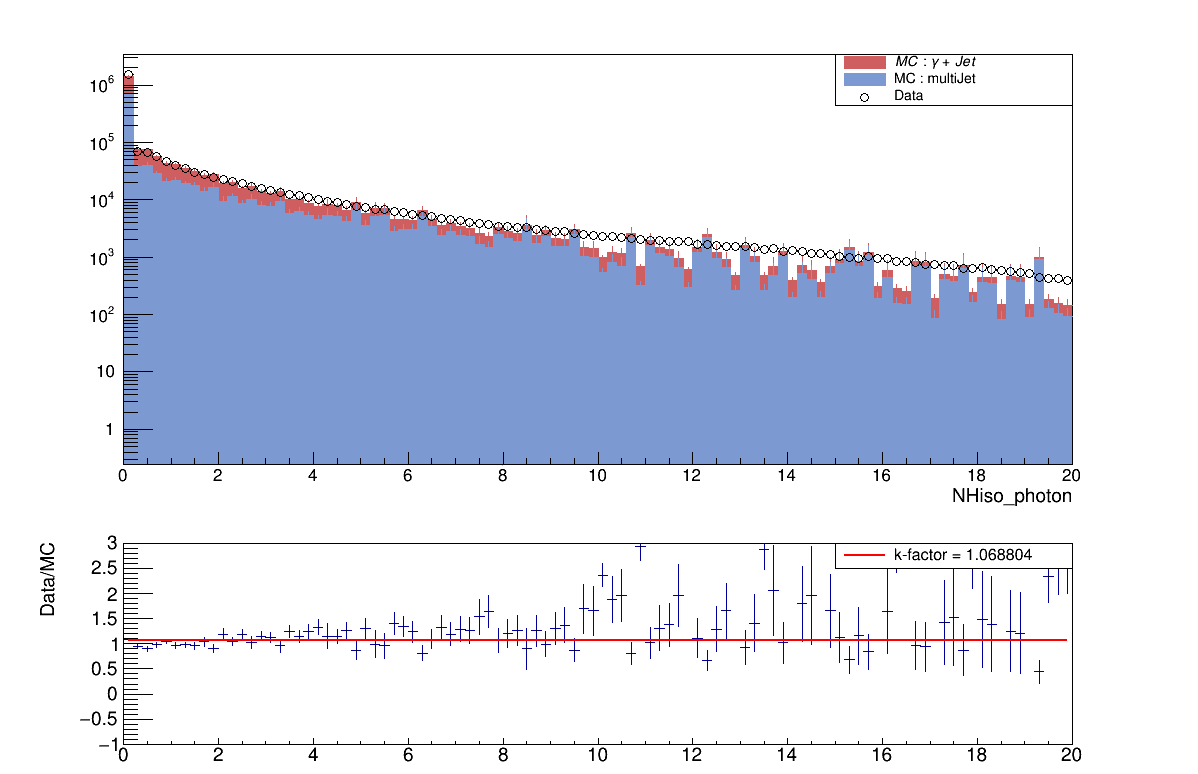
\includegraphics[width=0.8\textwidth]{NHiso_photon}\\[1cm]
  \caption{Top plot : Neutral hadron isolation variable for background (blue histogram) and signal MC (red histogram) and real data superimposed (empty circles). Normalized to integrated luminosity of $~36fb^{-1}$\\Bottom plot : Ratio of stacked background MC and signal MC over real data (blue cross) fitted by a constant (red line).}
  \label{NHiso_photon_dataVsMCbg}
\end{figure}

\section{Variable correlations}

%Training data needed-quantity increases with network complexity, so correlation between variables must be avoided in order to get the minimum redundancy.\\
Because we use distribution of the data in the control region as a proxy for their distribution in the signal region, we need to make sure that the variable for the sideband definition has low correlations with the other one. 
By looking at the correlation matrix (fig. \ref{corrMatrix_bgMC}) we can see that \emph{charged hadron isolation} is one good candidate and so will be used next for the sideband definition.\\

\begin{figure}[ht!]
  \centering
  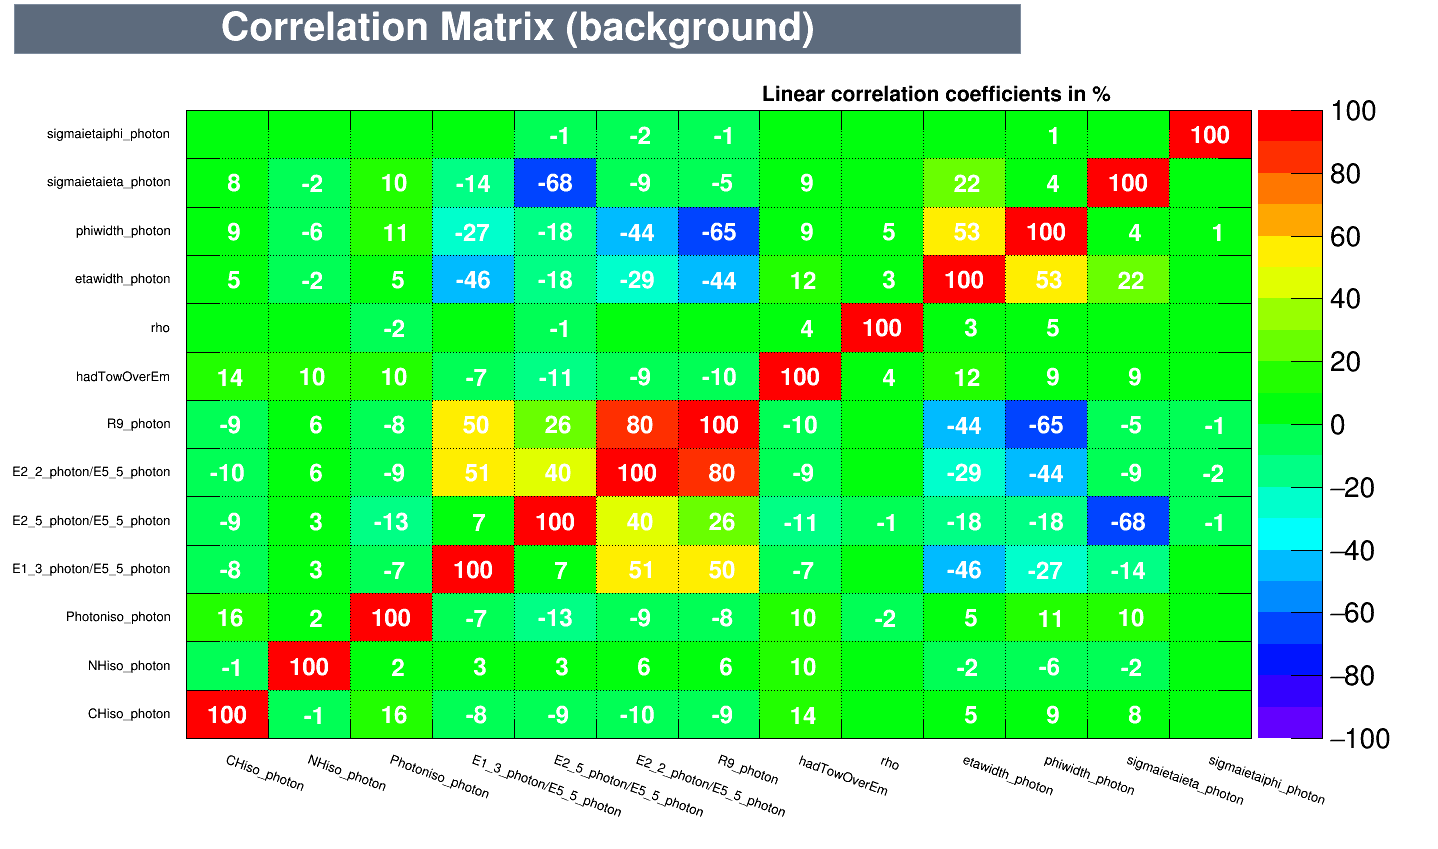
\includegraphics[width=0.7\textwidth]{corrMatrix_bgMC}\\[1cm]
  \caption{Correlation matrix for background MC, each line or column represent a variable.}
  \label{corrMatrix_bgMC}
\end{figure}

\section{Data driven background estimation}

MVA will be performed with real data for the background, thereby a sideband (background enriched region in the data sample) has to be defined on a low-correlated
variable.\emph{Charged hadron isolation} (fig. \ref{sideband}) has been chosen and the sideband defined in order to get the best ratio of background purity over number of events.
\begin{description}
	\item [Sideband definition]
	\begin{description}
    	\item 2.325 < \emph{Charge hadron isolation} < 15.
    	\item Background purity = 95.00 \%
		\item Number of events = $7.59*10^5$
	\end{description}
\end{description}

%Then a signal enriched region has been defined on the same variable, this cut will be applied on the signal data sample.
%\begin{description}
%	\item [Signal region definition]
%	\begin{description}
%    	\item \emph{Charge hadron isolation} < 2.
%    	\item Signal purity = ?? \%
%		\item Number of events = ??
%	\end{description}
%\end{description}

\begin{figure}[ht!]
  \centering
  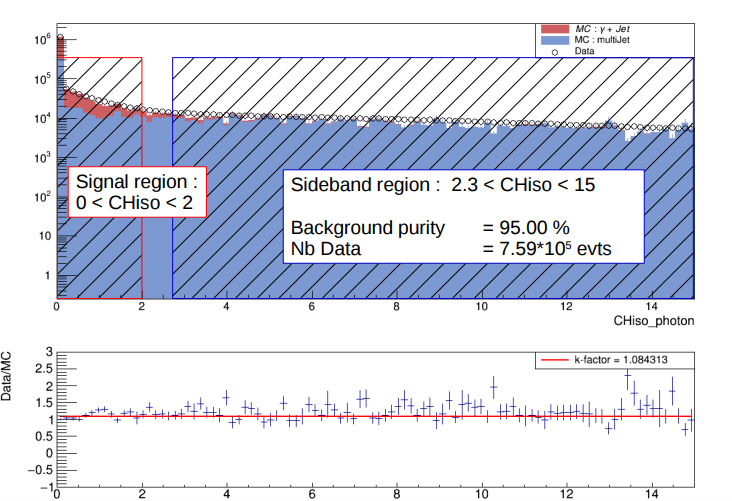
\includegraphics[width=0.7\textwidth]{sideband}\\[1cm]
  \caption{Charged hadron isolation for background MC (blue histogram), signal MC (red histogram) and real data superimposed (empty circles). Normalized to integrated luminosity of $~36fb^{-1}$\\On top of this is the sideband definition (red shaded area) and the signal region definition (blue shaded area)\\Bottom plot : Ratio of stacked background MC and signal MC over real data (blue cross) fitted by a constant (red line).}
  \label{sideband}
\end{figure}

For cross-check, we compare the variables shape for background MC and DATA in the sideband region.
(fig. \ref{MCbg_all_NHiso_photon}) shows an example of a comparison between \emph{neutral hadron isolation} for data in the sideband region and background Monte-Carlo. We can see a good agreement for MC and real data, except for a small trend in the high energy range probably due to the low statistics.
\begin{figure}[h!]
  \centering
  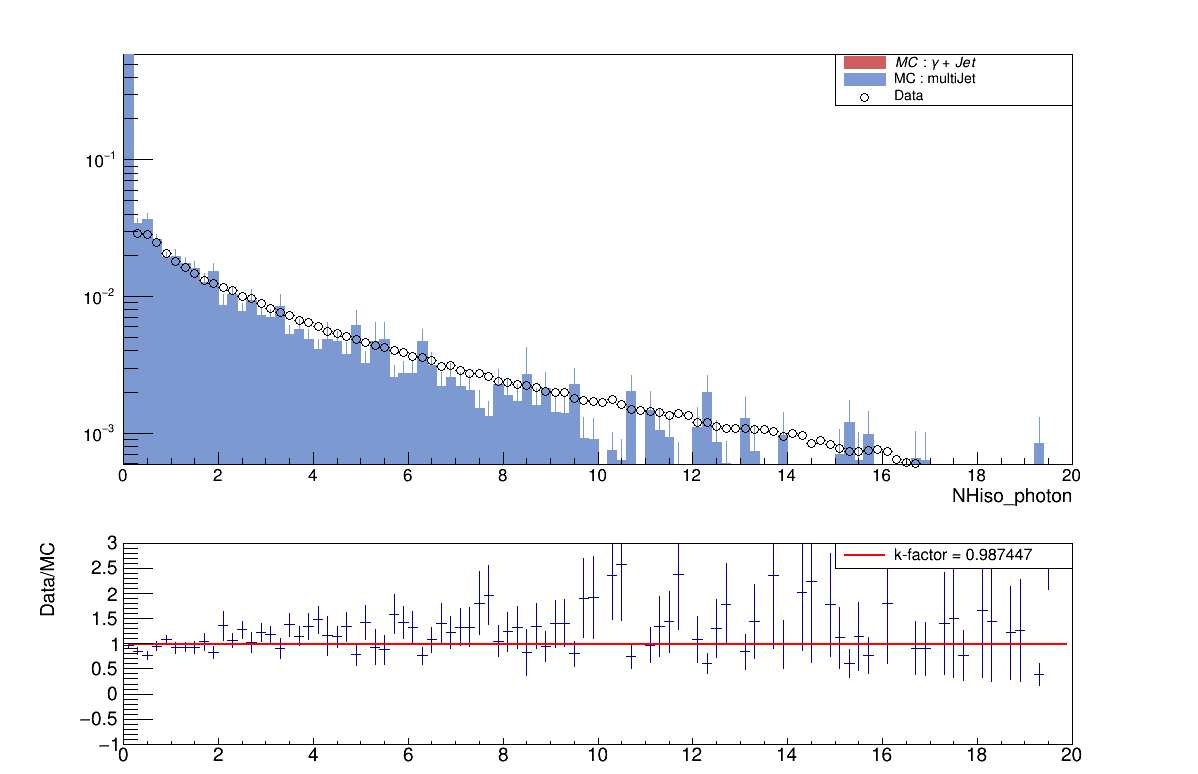
\includegraphics[width=0.7\textwidth]{MCbg_all_NHiso_photon}\\[1cm]
  \caption{Neutral hadron isolation for background MC (blue histogram) and real data in the sideband superimposed (empty circles). Normalized to 1.\\Bottom plot : Ratio of stacked background MC and signal MC over real data (blue cross) fitted by a constant (red line).}
  \label{MCbg_all_NHiso_photon}
\end{figure}

%%% Local Variables: 
%%% mode: latex
%%% TeX-master: "isae-report-template"
%%% End: 
